\documentclass[11pt]{article}\usepackage[]{graphicx}\usepackage[]{color}
%% maxwidth is the original width if it is less than linewidth
%% otherwise use linewidth (to make sure the graphics do not exceed the margin)
\makeatletter
\def\maxwidth{ %
  \ifdim\Gin@nat@width>\linewidth
    \linewidth
  \else
    \Gin@nat@width
  \fi
}
\makeatother

\definecolor{fgcolor}{rgb}{0.345, 0.345, 0.345}
\newcommand{\hlnum}[1]{\textcolor[rgb]{0.686,0.059,0.569}{#1}}%
\newcommand{\hlstr}[1]{\textcolor[rgb]{0.192,0.494,0.8}{#1}}%
\newcommand{\hlcom}[1]{\textcolor[rgb]{0.678,0.584,0.686}{\textit{#1}}}%
\newcommand{\hlopt}[1]{\textcolor[rgb]{0,0,0}{#1}}%
\newcommand{\hlstd}[1]{\textcolor[rgb]{0.345,0.345,0.345}{#1}}%
\newcommand{\hlkwa}[1]{\textcolor[rgb]{0.161,0.373,0.58}{\textbf{#1}}}%
\newcommand{\hlkwb}[1]{\textcolor[rgb]{0.69,0.353,0.396}{#1}}%
\newcommand{\hlkwc}[1]{\textcolor[rgb]{0.333,0.667,0.333}{#1}}%
\newcommand{\hlkwd}[1]{\textcolor[rgb]{0.737,0.353,0.396}{\textbf{#1}}}%
\let\hlipl\hlkwb

\usepackage{ulem}

\usepackage{framed}
\makeatletter
\newenvironment{kframe}{%
 \def\at@end@of@kframe{}%
 \ifinner\ifhmode%
  \def\at@end@of@kframe{\end{minipage}}%
  \begin{minipage}{\columnwidth}%
 \fi\fi%
 \def\FrameCommand##1{\hskip\@totalleftmargin \hskip-\fboxsep
 \colorbox{shadecolor}{##1}\hskip-\fboxsep
     % There is no \\@totalrightmargin, so:
     \hskip-\linewidth \hskip-\@totalleftmargin \hskip\columnwidth}%
 \MakeFramed {\advance\hsize-\width
   \@totalleftmargin\z@ \linewidth\hsize
   \@setminipage}}%
 {\par\unskip\endMakeFramed%
 \at@end@of@kframe}
\makeatother

\definecolor{shadecolor}{rgb}{.97, .97, .97}
\definecolor{messagecolor}{rgb}{0, 0, 0}
\definecolor{warningcolor}{rgb}{1, 0, 1}
\definecolor{errorcolor}{rgb}{1, 0, 0}
\newenvironment{knitrout}{}{} % an empty environment to be redefined in TeX

\usepackage{xcolor}
\usepackage{alltt}
\usepackage{graphicx, fancyhdr}
\usepackage{amsmath, amsfonts}
\usepackage{color}
\usepackage{hyperref}

\newcommand{\blue}[1]{{\color{blue} #1}}

\setlength{\topmargin}{-.5 in} 
\setlength{\textheight}{9 in}
\setlength{\textwidth}{6.5 in} 
\setlength{\evensidemargin}{0 in}
\setlength{\oddsidemargin}{0 in} 
\setlength{\parindent}{0 in}
\newcommand{\ben}{\begin{enumerate}}
\newcommand{\een}{\end{enumerate}}


\lhead{STAT 305}
\chead{Homework 3} 
\rhead{Due Thursday, February $6^{th}$ in the class}
\lfoot{Spring 2020} 
\cfoot{\thepage} 
 
\renewcommand{\headrulewidth}{0.4pt} 
\renewcommand{\footrulewidth}{0.4pt} 

\def\Exp#1#2{\ensuremath{#1\times 10^{#2}}}
\def\Case#1#2#3#4{\left\{ \begin{tabular}{cc} #1 & #2 \phantom
{\Big|} \\ #3 & #4 \phantom{\Big|} \end{tabular} \right.}
\IfFileExists{upquote.sty}{\usepackage{upquote}}{}
\usepackage{Sweave}
\begin{document}
\Sconcordance{concordance:stat305-hw3_s20_sol.tex:stat305-hw3_s20_sol.Rnw:%
1 84 1 1 0 32 1 1 6 1 3 3 1 1 22 33 1 1 11 1 2 100 1 1 3 1 2 2 1 1 13 1 %
2 3 1 1 12 1 2 5 1}

\pagestyle{fancy} 

Show \textbf{all} of your work on this assignment and answer each question fully in the given context. 

\vspace{0.3cm}

\textbf{If you cannot submit your homework in the class, you can drop it at my office door in 3220 Snedecore Hall by Thursday at 03:30 PM.}

\vspace{0.3cm}

\textcolor{red}{In this homework, you CAN use JMP to plot the data whenever it is asked in the question.}
\vspace{0.3cm}

\emph{Please} staple your assignment and write your name !

\begin{enumerate}
\item \textbf{[Ch 3, Exercise 8, pg. 116]} Back to problem 5 of homework two,  the accompanying data are the times to failure (in millions of cycles) of high-speed turbine engine bearings made out of two different compounds. These were taking from "Analysis of Single Classification Experiments Based on Censored Samples from the Two-parameter Weibull Distribution" by J. I. McCool (*The Journal of Statistical Planning and Inference*, 1979).
    

\begin{center}
	\begin{tabular}{|ccccccccccc|}	
		\hline
		compound_1  & 3.03 & 5.53 & 5.60 & 9.30 & 9.92 & 12.51 & 12.95 & 15.21 & 16.04 & 16.84\\
		compound_2 & 3.19 & 4.26 & 4.47 & 4.53 & 4.67 & 4.69 & 5.78 & 6.79 & 9.37 & 12.75\\
		\hline
	\hline                 
	\end{tabular}
\end{center}

\begin{enumerate}
    \item Plot a side-by-side boxplot of the two compounds.[10 pts]\\
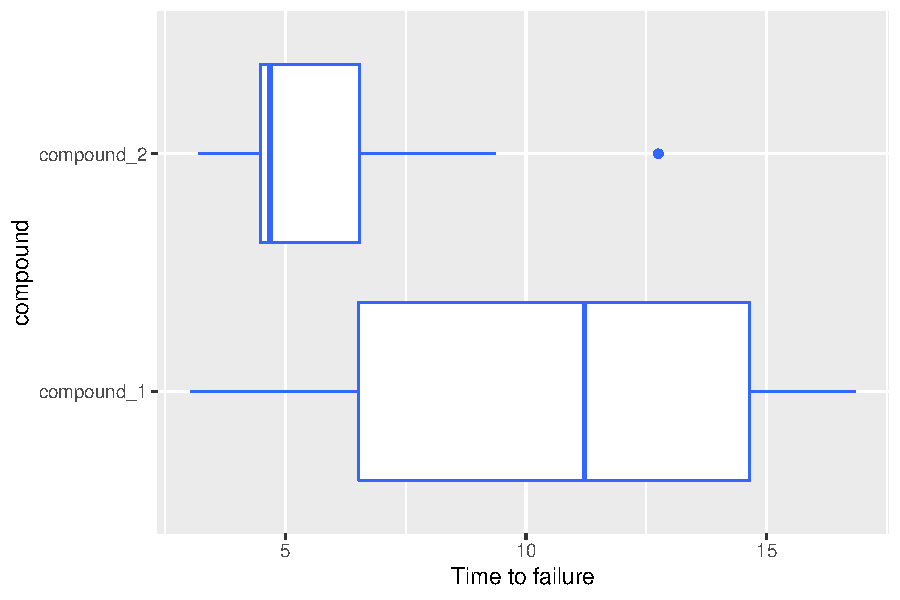
\includegraphics{stat305-hw3_s20_sol-001}
    
    
    \item Find all quantiles of compound 1 and use Normal quantile table attached to this homework to find the corresponding normal quantiles[10 pts]\\
    

    \emph{hint} This part is similar to what we did in class working on ch 3 handout. \\

\begin{center}
\begin{tabular}{r|r|r|r}
\hline
i & p=$\frac{i-.5}{10}$ & compound_1 quantiles & Standard Normal quantiles\\
\hline
1 & 0.05 & 3.03 & -1.6448536\\
\hline
2 & 0.15 & 5.53 & -1.0364334\\
\hline
3 & 0.25 & 5.60 & -0.6744898\\
\hline
4 & 0.35 & 9.30 & -0.3853205\\
\hline
5 & 0.45 & 9.92 & -0.1256613\\
\hline
6 & 0.55 & 12.51 & 0.1256613\\
\hline
7 & 0.65 & 12.95 & 0.3853205\\
\hline
8 & 0.75 & 15.21 & 0.6744898\\
\hline
9 & 0.85 & 16.04 & 1.0364334\\
\hline
10 & 0.95 & 16.84 & 1.6448536\\
\hline
\end{tabular}
\end{center}

    \item Using the results in part b, plot theoretical Normal QQ-plot against quantiles of compound 1.[10 pts]
    
    
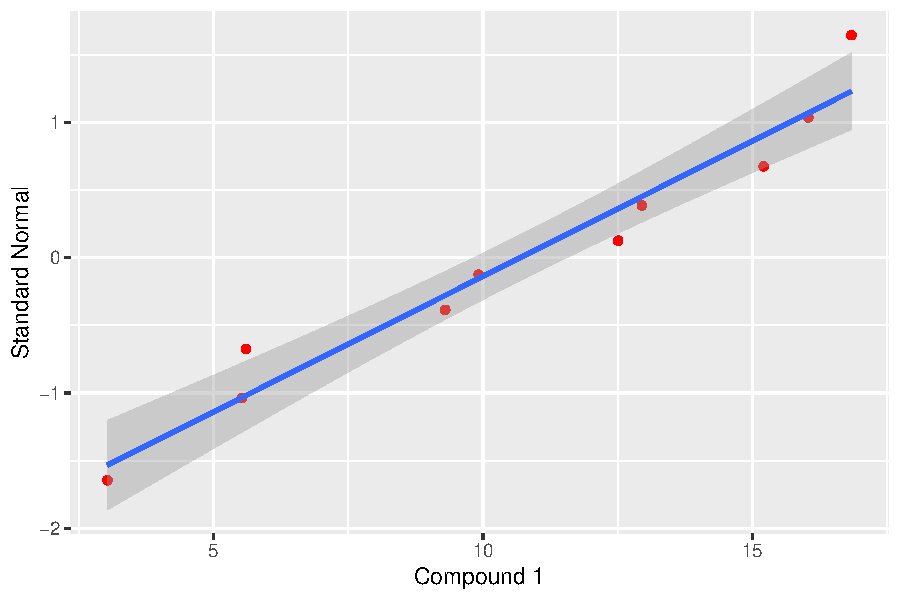
\includegraphics{stat305-hw3_s20_sol-003}
    
    \item Using the theoretical Normal quantile plot in part c, what can we say about the shape and distribution of compound 2 data? [5 pts]\\
   \emph{Solution:} It seems the data of compound 1 have bell-shaped distribution, so they are pretty normal.
    \item Give the coordinates  of the upper right point that would appear on a regular graph paper. Also, give the coordinates of the lower left point that would appear on a normal plot of the compound 2 data. [5 pts]\\
    \emph{Solution:} coordinates  of the upper right point on a regular graph paper: $(0.95, 16.84)$\\
    coordinates  of the lower left point on a normal graph paper: $(0.05, -1.645)$
\end{enumerate}    


\item Calculate the sample mean and sample variance for the following samples:
\begin{enumerate}
	\item Sample 1: -1.05, -1.0, -0.5, 0.15, 0.6, 0.65, 0.7, 1.25 [5 pts]
	\item Sample 2: -2.1, -2.0, -1.0, 0.3, 1.2, 1.3, 1.4, 2.5 [5 pts]
\end{enumerate}
\emph{Solution:}For sample 1:
    \begin{align*}
    	\bar{x} &= \frac{1}{n}\sum_{i=1}^{n}x_i\\
    			&= \frac{1}{8}\sum_{i=1}^{8}x_i= \frac{1}{8} (-1.05 + (-1.0)+ (-0.5) + 0.15 + 0.6 + 0.65+ 0.7+ 1.25) \\
    			&= 0.1\\
    	s^2 &= \frac{1}{n-1}\sum_{i=1}^5 (x_i - \bar{x})^2 \\
    		&= \frac{1}{n-1}( (x_1 - \bar{x})^2 + (x_2 - \bar{x})^2 + (x_3 - \bar{x})^2 + (x_4 - \bar{x})^2 + (x_5 - \bar{x})^2+ (x_6 - \bar{x})^2+ (x_7 - \bar{x})^2\\
    		&+ (x_8 - \bar{x})^2  )\\
    		&= \frac{1}{8}( (-1.05 -0.1)^2 + (-1.0 - 0.1)^2+ (-0.5 - 0.1)^2+ (0.15 - 0.1)^2+ (0.6 - 0.1)^2\\
    		&+ (0.65 - 0.1)^2+ (0.7 - 0.1)^2+ (1.25 - 0.1)^2  )\\
    		&= 0.73\\
    	s&= \sqrt{s^2}= 0.85
    \end{align*}

For sample 2:
    \begin{align*}
    	\bar{x} &= \frac{1}{n}\sum_{i=1}^{n}x_i\\
    	&= \frac{1}{8}\sum_{i=1}^{8}x_i= \frac{1}{8} (-2.1+ (-2.0)+ (-1.0)+ 0.3+ 1.2+ 1.3+ 1.4+ 2.5) \\
    	&= 0.2\\
    	s^2 &= \frac{1}{n-1}\sum_{i=1}^5 (x_i - \bar{x})^2 \\
    	&= \frac{1}{n-1}( (x_1 - \bar{x})^2 + (x_2 - \bar{x})^2 + (x_3 - \bar{x})^2 + (x_4 - \bar{x})^2 + (x_5 - \bar{x})^2+ (x_6 - \bar{x})^2+ (x_7 - \bar{x})^2\\
    	&+ (x_8 - \bar{x})^2  )\\
    	&= \frac{1}{8}( (-2.1 -0.2)^2 + ( -2.0 - 0.2)^2+ (-1.0 - 0.2)^2+ (0.3 - 0.2)^2+ (1.2 - 0.2)^2\\
    	&+ (1.3 - 0.2)^2+ (1.4 - 0.2)^2+ (2.5 - 0.2)^2  )\\
    	&= 2.93\\
    	s&= \sqrt{s^2}= 1.71
    \end{align*}

\item  Mechanical engineers were interested in studying the effects of 2 chemical compounds 
	(low Ca, high Ca) and 3 uni-axial pressure (P1, P2, P3) on metal bars lifetime. A total of 12 specimen were assigned to the possible combinations with two metal bars in each treatment. The lifetime of the bars were recorded after each run of the experiment. 
\begin{enumerate}
	\item How many possible combinations of $compound$ $\times{ pressure}$ are there available for a full factorial study? Draw a table for this design to get full credit.[5 pts]
\textbf{Solution:} There are $2\times{3} = 6$ possible combinations for a full factorial study. The following table shows a full factorial study with two specimen per treatment.
	\begin{center}
			\begin{tabular}{|c|c|c|c|}
				\hline
				& P1 & P2 &P3\\
				\hline
				Low Ca & $||$ &$||$ &$||$ \\
				\hline
				High Ca &$||$ &$||$ & $||$\\
				\hline
			\end{tabular}
	\end{center}
	
	\item What is the response variable in this study?[2 pts]\\
	\textbf{Solution:} The response variable is the metal bars lifetime
	\item What are experimental variables in this study? [2 pts]\\
	\textbf{Solution:} The chemical compound and uni-axial pressure are the experimental variables. 
	\item What type of experimental variables are they in part 3 above?(Be careful with this question, we already know they are experimental variables and not response variable)[2 pts]\\
	\textbf{Solution:} The chemical compound and uni-axial pressure are both \textbf{qualitative (categorical)} variables. 
	\item For this full factorial study with two factors chemical compounds and uni-axial pressure, the six experimental runs are labeled as:
	
	No. 1:  low- P1, \hspace{0.5cm} No. 2:  low-P2,
	\hspace{0.5cm} No. 3: low-P3, \\  No. 4:  high- P1,
	\hspace{0.5cm} No. 5:  high- P2, \hspace{0.1 cm}and
	\hspace{0.1cm} No. 6:  high- P3.
	
	\noindent Based on the following random digits
	
	\hspace{3.5cm}$49502 \; 18963 \; 63920 \; 39544 \; 25804$\\
	Which experiment should be done last?[4 pts]\\
	\textbf{Solution:} This exercise directly asks to use a random number table to randomly run the experiments. Using the digits, experimental run \textbf{NO. 3} will be the last to do. 
\end{enumerate}

\item \textbf{JMP assignment: chapter 3 section 2 problem 2 page 92}

Using the data of two turbin suppliers companies below, answer the questions using JMP.

\begin{center}
	\begin{tabular}{|cc|}	
		\hline
		Suplier I & Suplier II\\
		\hline
		0.52 & 0.89 \\
		0.37 & 0.99 \\ 
		0.92 & 1.45     \\
		2.89 & 1.47     \\
	    3.62 & 1.58     \\
	    0.65 & 2.27     \\
 
	\hline                 
	\end{tabular}
\end{center}
   \begin{enumerate}
         \item Provide a scatter plot  for the two data sets. [10 pts] \\
         \textbf{Solution:}
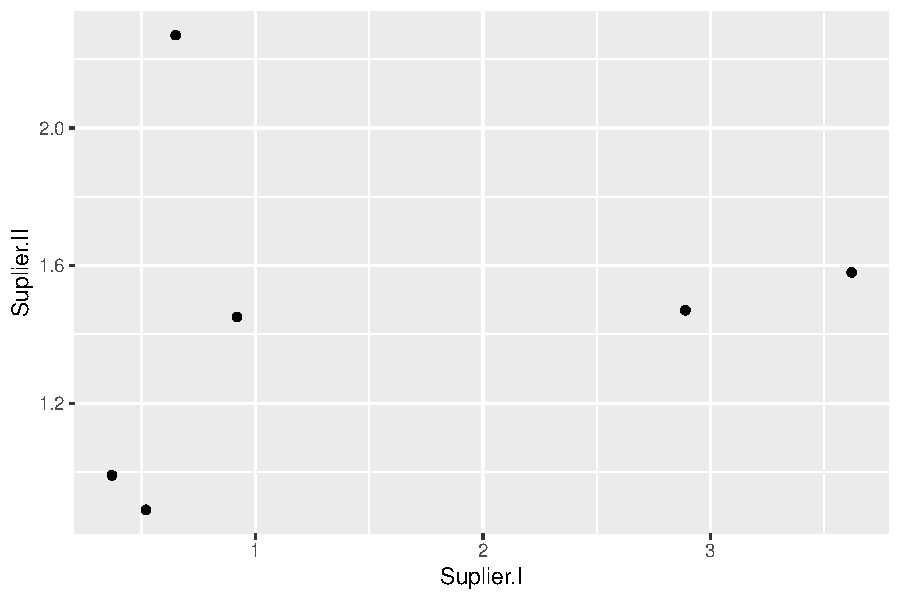
\includegraphics{stat305-hw3_s20_sol-004}

         \item Plot a Normal QQ-plot of the supplier I data and interpret the shape and distribution of supplier I data.[5 pts]\\
         \textbf{Solution:}
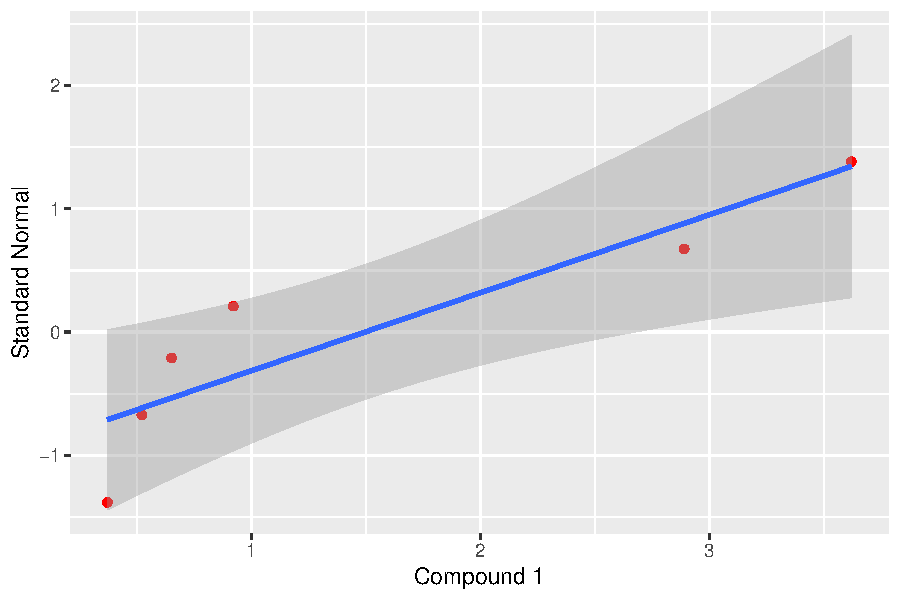
\includegraphics{stat305-hw3_s20_sol-005}
   The data from suplier I does not have a bell-shaped distribution  because it does not follow a normal distribution as the points do not lie around the straight line in normal QQ-plot.      
         \item Plot a Normal QQ-plot of the supplier II data and interpret the shape and distribution of supplier II data.[5 pts]\\
         \textbf{Solution:}
\begin{center}
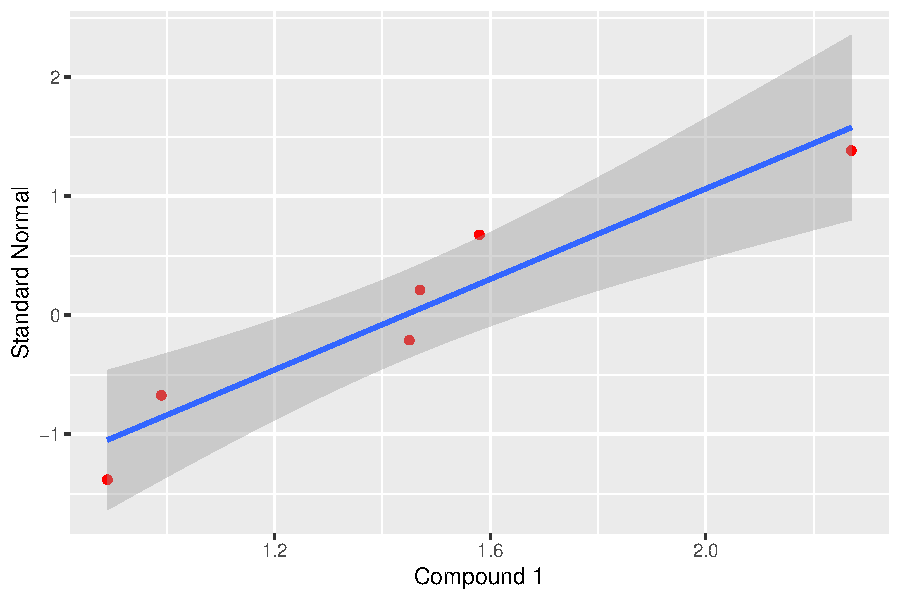
\includegraphics{stat305-hw3_s20_sol-006}
\end{center}
   The data from suplier II does not seem to have a bell-shaped distribution because its quantiles  do not  follow a normal distribution as the points do  lie around the straight line in normal QQ-plot.
   \end{enumerate}

\emph{Total: 85 pts}
\end{document}
